\newcommand{\op}[1]{\operatorname{#1}}
\newcommand{\mbf}[1]{\mathbf{#1}}

\section{Method}

\begin{figure}[h]
\begin{center}
\begin{tabular}{c}
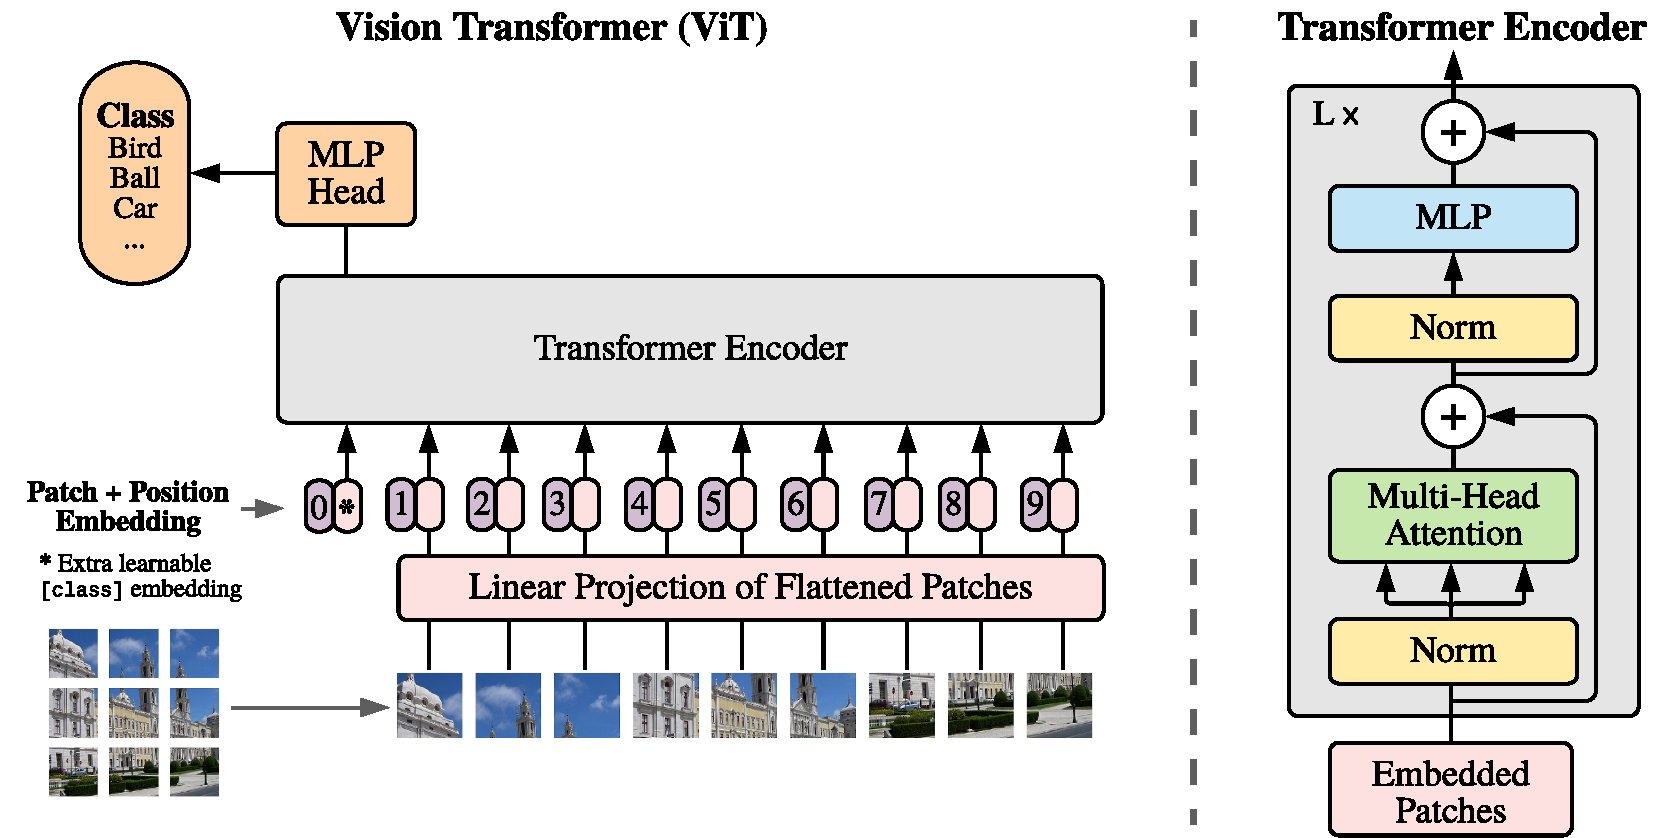
\includegraphics[width=.83\textwidth]{images/model_scheme.pdf}
\end{tabular}
\end{center}
\caption{Model overview. We split an image into fixed-size patches, linearly embed each of them, add position embeddings, and feed the resulting sequence of vectors to a standard Transformer encoder. In order to perform classification, we use the standard approach of adding an extra learnable ``classification token'' to the sequence. The illustration of the Transformer encoder was inspired by \citet{vaswani2017}.}
\label{fig:model}
\end{figure}

In model design we follow the original Transformer \citep{vaswani2017} as closely as possible. 
An advantage of this intentionally simple setup is that scalable NLP Transformer architectures -- and their efficient implementations -- can be used almost out of the box.

\subsection{\oursfull{} (\oursabbrv{})}\label{sec:patch_transformer}

An overview of the model is depicted in Figure~\ref{fig:model}.
The standard Transformer receives as input a 1D sequence of token embeddings.
To handle 2D images, we reshape the image $\mbf{x} \in \mathbb{R}^{H \times W \times C}$ into a sequence of flattened 2D patches $\mbf{x}_p \in \mathbb{R}^{N \times (P^2 \cdot C)}$, where $(H, W)$ is the resolution of the original image, $C$ is the number of channels, $(P,P)$ is the resolution of each image patch, and $N=HW/P^2$ is the resulting number of patches, which also serves as the effective input sequence length for the Transformer.
The Transformer uses constant latent vector size $D$ through all of its layers, so we flatten the patches and map to $D$ dimensions with a trainable linear projection (Eq.~\ref{eq:embedding}).
We refer to the output of this projection as the patch embeddings.

Similar to BERT's \verb|[class]| token, we prepend a learnable embedding to the sequence of embedded patches ($\mbf{z}_0^0=\mbf{x}_\text{class}$), whose state at the output of the Transformer encoder ($\mbf{z}^0_L$) serves as the image representation $\mbf{y}$ (Eq.~\ref{eq:final_rep}). 
Both during pre-training and fine-tuning, a classification head is attached to $\mbf{z}^0_L$.
The classification head is implemented by a MLP with one hidden layer at pre-training time and by a single linear layer at fine-tuning time.

Position embeddings are added to the patch embeddings to retain positional information.
We use standard learnable 1D position embeddings, since we have not observed significant performance gains from using more advanced 2D-aware position embeddings  (Appendix~\ref{app:pos_emb}).
The resulting sequence of embedding vectors serves as input to the encoder.

The Transformer encoder \citep{vaswani2017} consists of alternating layers of multiheaded self-attention (MSA, see Appendix~\ref{sec:self_attention}) and MLP blocks (Eq.~\ref{eq:msa_apply}, \ref{eq:mlp_apply}).
Layernorm (LN) is applied before every block, and residual connections after every block \citep{wang2019-preLN,Baevski2019Adaptive}.
The MLP contains two layers with a GELU non-linearity.
\begin{align}
    \mbf{z}_0 &= [ \mbf{x}_\text{class}; \, \mbf{x}^1_p \mbf{E}; \, \mbf{x}^2_p \mbf{E}; \cdots; \, \mbf{x}^{N}_p \mbf{E} ] + \mbf{E}_{pos},
    && \mbf{E} \in \mathbb{R}^{(P^2 \cdot C) \times D},\, \mbf{E}_{pos}  \in \mathbb{R}^{(N + 1) \times D} \label{eq:embedding} \\
    \mbf{z^\prime}_\ell &= \op{MSA}(\op{LN}(\mbf{z}_{\ell-1})) + \mbf{z}_{\ell-1}, && \ell=1\ldots L \label{eq:msa_apply} \\
    \mbf{z}_\ell &= \op{MLP}(\op{LN}(\mbf{z^\prime}_{\ell})) + \mbf{z^\prime}_{\ell}, && \ell=1\ldots L  \label{eq:mlp_apply} \\
    \mbf{y} &= \op{LN}(\mbf{z}_L^0) \label{eq:final_rep}
\end{align}

\paragraph{Inductive bias.} 
We note that Vision Transformer has much less image-specific inductive bias than CNNs. 
In CNNs, locality, two-dimensional neighborhood structure, and translation equivariance are baked into each layer throughout the whole model. 
In ViT, only MLP layers are local and translationally equivariant, while the self-attention layers are global. 
The two-dimensional neighborhood structure is used very sparingly: in the beginning of the model by cutting the image into patches and at fine-tuning time for adjusting the position embeddings for images of different resolution (as described below).
Other than that, the position embeddings at initialization time carry no information about the 2D positions of the patches and all spatial relations between the patches have to be learned from scratch.

\paragraph{Hybrid Architecture.}
As an alternative to raw image patches, the input sequence can be formed from feature maps of a CNN~\citep{LeCun1989BackpropagationAT}.
In this hybrid model, the patch embedding projection $\mbf{E}$  (Eq.~\ref{eq:embedding}) is applied to patches extracted from a CNN feature map.
As a special case, the patches can have spatial size 1x1, which means that the input sequence is obtained by simply flattening the spatial dimensions of the feature map and projecting to the Transformer dimension.  
The classification input embedding and position embeddings are added as described above.

\subsection{Fine-tuning and Higher Resolution}

Typically, we pre-train ViT on large datasets, and fine-tune to (smaller) downstream  tasks.
For this, we remove the pre-trained prediction head and attach a zero-initialized $D\times K$ feedforward layer, where $K$ is the number of downstream classes.
It is often beneficial to fine-tune at higher resolution than pre-training~\citep{touvron2019,kolesnikov2020-bit}.
When feeding images of higher resolution, we keep the patch size the same, which results in a larger effective sequence length.
The \oursfull{} can handle arbitrary sequence lengths (up to memory constraints), however, the pre-trained position embeddings may no longer be meaningful.
We therefore perform 2D interpolation of the pre-trained position embeddings, according to their location in the original image.
Note that this resolution adjustment and patch extraction are the only points at which an inductive bias about the 2D structure of the images is manually injected into the \oursfull{}.

